%% Week 42 -- lecture slides for the 2x45 min Monday lecture (version 2).
%% Division of labour: the slides set up each question and show the final
%% result and the evidence (figures, numbers); the derivations are done on
%% the blackboard.  Blue "On the board" boxes mark where the lecturer turns
%% to the board; the result appears on the next click.  The board work is
%% written out in week42monday_whiteboard_v2.md (sections W1-W6).
%% The full version with all details and code is week42monday.tex.
%% Figures: ./figures/v2_*.png, made by make_week42_v2_figures.py and
%% make_week42_v2_de_figures.py from the code in week42monday.ipynb.
%% Build:  tectonic week42monday_lecture_v2.tex   (or pdflatex twice)
\documentclass[10pt,aspectratio=169]{beamer}
\usetheme{red_plain}
\usepackage[T1]{fontenc}
\usepackage[utf8]{inputenc}
\usepackage{amsmath,amssymb,bm}
\usepackage{graphicx}
\usepackage{xcolor}
\usepackage{booktabs}
\usepackage{tikz}
\usetikzlibrary{arrows.meta,positioning}
\graphicspath{{./figures/}}

%% ---- short questions to the audience
\newcommand{\question}[1]{\begin{block}{Question}#1\end{block}}
\newcommand{\answer}[1]{\pause\begin{block}{Answer}#1\end{block}}
\newcounter{quickq}
\newenvironment{quickq}[1][]{%
  \stepcounter{quickq}%
  \begin{frame}{Quick question \arabic{quickq}: #1}%
  \setbeamercolor{block title}{bg=structure.fg,fg=white}%
  \setbeamercolor{block body}{bg=structure.fg!8}%
  \small
}{\end{frame}}

%% ---- "On the board" box: what is derived by hand at this point
\definecolor{boardblue}{rgb}{0.10,0.25,0.55}
\newenvironment{boardbox}[1]{%
  \setbeamercolor{block title}{bg=boardblue,fg=white}%
  \setbeamercolor{block body}{bg=boardblue!8}%
  \begin{block}{On the board (#1)}}{\end{block}}

\setbeamertemplate{footline}[frame number]
\setbeamertemplate{blocks}[rounded][shadow=false]
\setbeamercovered{invisible}

\title{Week 42: From Backpropagation to Differential Equations}
\author{Morten Hjorth-Jensen \\ Viktor Svensson}
\institute{Department of Physics and Center for Computing in Science Education,\\
  University of Oslo, Norway}
\date{}

\begin{document}

\begin{frame}
\titlepage
\end{frame}

\begin{frame}{Plan for today}
\begin{columns}[T]
\begin{column}{0.48\textwidth}
\begin{block}{First hour}
\begin{enumerate}
  \item \textbf{Backpropagation}: the chain rule, organised
  \item \textbf{Activation and cost functions}: why they come in pairs
  \item \textbf{Universal approximation}: what a network can represent
\end{enumerate}
\end{block}
\end{column}
\begin{column}{0.48\textwidth}
\begin{block}{Second hour}
\begin{enumerate}
  \setcounter{enumi}{3}
  \item \textbf{Neural networks for differential equations}
  \begin{itemize}
    \item the equation as the cost
    \item why the activation function matters
    \item boundary conditions
    \item pros and cons vs.\ standard methods
  \end{itemize}
\end{enumerate}
\end{block}
\end{column}
\end{columns}
\vspace{8pt}
\begin{boardbox}{take notes}
Most derivations today are done on the blackboard.  The slides give the
setup and the results.
\end{boardbox}
\small
\textbf{Tuesday:} backpropagation in code.  \textbf{Exercises week 42:}
deadline Friday October 16.
\end{frame}

%% ====================================================================
%% Part 1: backpropagation
%% ====================================================================

\section{Backpropagation}

\begin{frame}{Recap: the forward pass}
\begin{columns}[c]
\begin{column}{0.45\textwidth}
\centering
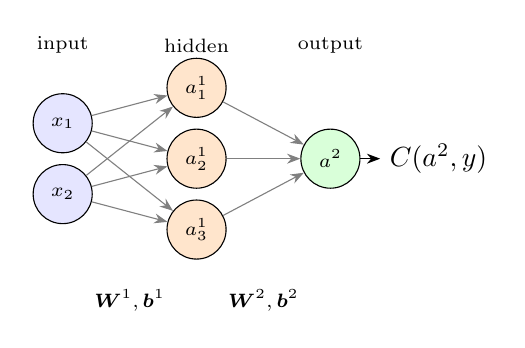
\begin{tikzpicture}[x=1.7cm,y=0.9cm,
    neuron/.style={circle,draw,minimum size=0.75cm,inner sep=0pt,font=\scriptsize},
    >=Stealth]
  \foreach \i in {1,2} \node[neuron,fill=blue!10] (x\i) at (0,-\i-0.5) {$x_{\i}$};
  \foreach \j in {1,2,3} \node[neuron,fill=orange!20] (h\j) at (1,-\j) {$a^1_{\j}$};
  \node[neuron,fill=green!15] (o) at (2,-2) {$a^2$};
  \node[right=0.25cm of o] (C) {$C(a^2,y)$};
  \foreach \i in {1,2} \foreach \j in {1,2,3} \draw[->,gray] (x\i) -- (h\j);
  \foreach \j in {1,2,3} \draw[->,gray] (h\j) -- (o);
  \draw[->] (o) -- (C);
  \node[font=\scriptsize] at (0.5,-4.0) {$\bm{W}^1,\bm{b}^1$};
  \node[font=\scriptsize] at (1.5,-4.0) {$\bm{W}^2,\bm{b}^2$};
  \node[font=\scriptsize] at (0,-0.4) {input};
  \node[font=\scriptsize] at (1,-0.4) {hidden};
  \node[font=\scriptsize] at (2,-0.4) {output};
\end{tikzpicture}
\end{column}
\begin{column}{0.53\textwidth}
One sample $\bm{x}$, layers $l=1,\dots,L$, $\bm{a}^{0}=\bm{x}$:
\[
  \boxed{\;\bm{z}^{l}=\bm{W}^{l}\bm{a}^{l-1}+\bm{b}^{l},\qquad
  \bm{a}^{l}=f(\bm{z}^{l})\;}
\]
\small
\begin{itemize}
  \item $\bm{W}^{l}$ has shape (nodes out, nodes in)
  \item $f$ acts element by element; the last layer has its own
        \emph{output} activation
  \item the cost $C$ compares the output $\bm{a}^{L}$ with the target
        $\bm{y}$
\end{itemize}
\vspace{4pt}
\footnotesize In code with many samples we stack them as rows,
$\bm{Z}^{l}=\bm{A}^{l-1}\bm{W}^{l}+\bm{b}^{l}$: the same equations,
transposed.
\end{column}
\end{columns}
\end{frame}

\begin{frame}{The four equations of backpropagation}
\begin{columns}[T]
\begin{column}{0.52\textwidth}
\small
We want $\partial C/\partial w^{l}_{jk}$ and $\partial C/\partial b^{l}_{j}$
for every layer.  Key quantity: the \emph{error} of node $j$ in layer $l$,
\[
  \delta^{l}_{j}=\frac{\partial C}{\partial z^{l}_{j}}.
\]
\begin{boardbox}{W1}
Use the chain rule to find $\delta^{L}$, then $\delta^{l}$ from
$\delta^{l+1}$, then the gradients.  Note: node $j$ in layer $l$ feeds
\emph{every} node in layer $l+1$.
\end{boardbox}
\end{column}
\begin{column}{0.46\textwidth}
\pause
\begin{block}{Result ($\circ$: element-wise product)}
\vspace{-6pt}
\begin{align*}
  \bm{\delta}^{L}&=f'(\bm{z}^{L})\circ\frac{\partial C}{\partial\bm{a}^{L}}\\
  \bm{\delta}^{l}&=\bigl((\bm{W}^{l+1})^{T}\bm{\delta}^{l+1}\bigr)\circ f'(\bm{z}^{l})\\
  \frac{\partial C}{\partial\bm{b}^{l}}&=\bm{\delta}^{l},\qquad
  \frac{\partial C}{\partial\bm{W}^{l}}=\bm{\delta}^{l}\,(\bm{a}^{l-1})^{T}
\end{align*}
\end{block}
\small
\begin{itemize}
  \item Start at the output, go \emph{backwards}.  Each $\bm{\delta}^{l}$
        reuses $\bm{\delta}^{l+1}$.
  \item Weight gradient $=$ error at the node it goes \emph{into} $\times$
        signal from the node it comes \emph{from}.
  \item The error is multiplied by $f'$ in every layer.
\end{itemize}
\end{column}
\end{columns}
\end{frame}

%% ====================================================================
%% Part 2: activation functions and cost functions
%% ====================================================================

\section{Activation and cost functions}

\begin{frame}{Hidden activation functions}
\centering
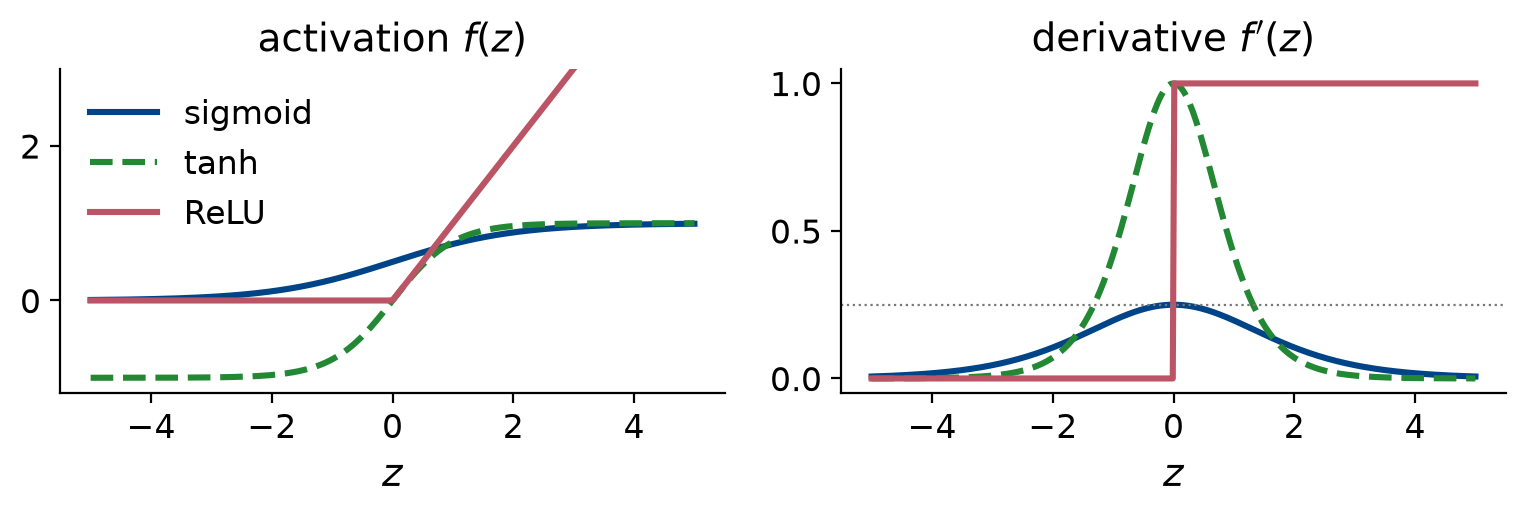
\includegraphics[width=0.78\textwidth]{v2_activations}\par
\vspace{2pt}
\raggedright\small
\begin{columns}[T]
\begin{column}{0.33\textwidth}
\textbf{Sigmoid} $\sigma(z)=\frac{1}{1+e^{-z}}$\\
$\sigma'=\sigma(1-\sigma)\le\frac14$.\\
Flat ($\sigma'\approx0$) for large $|z|$.
\end{column}
\begin{column}{0.33\textwidth}
\textbf{tanh}\\
$\tanh'=1-\tanh^{2}\le1$.\\
Centred at zero; also flat for large $|z|$.
\end{column}
\begin{column}{0.33\textwidth}
\textbf{ReLU} $\max(0,z)$\\
$f'=1$ for $z>0$, $0$ otherwise.  A unit with $z<0$ for all inputs never
learns (``dead'').
\end{column}
\end{columns}
\vspace{4pt}
\begin{block}{What matters}
$f$ must be \textbf{non-linear}: otherwise the whole network is a single
linear map.  For training, $f'$ matters.  Backpropagation multiplies by
$f'$ once per layer, so with $L$ sigmoid layers the error shrinks by up to
$(\tfrac14)^{L}$: the \emph{vanishing gradient}.  This is why ReLU is the
default in deep networks.
\end{block}
\end{frame}

\begin{frame}{Initialising the weights}
\begin{columns}[T]
\begin{column}{0.5\textwidth}
\small
\textbf{Not all equal} (e.g.\ all zero): then every unit in a layer computes
the same thing, gets the same gradient, and stays identical.  Random
weights break the symmetry.\\[4pt]
\textbf{The scale matters.}  With $M$ inputs per node and weights of
variance $\sigma_w^{2}$:
\[
  \operatorname{Var}(z)\approx M\,\sigma_w^{2}\,\overline{a^{2}}
\]
\begin{itemize}
  \item $\sigma_w$ too large: $|z|$ large, tanh/sigmoid saturate,
        gradients blow up or die.
  \item $\sigma_w$ too small: the signal shrinks in every layer, and so do
        the gradients.
\end{itemize}
\end{column}
\begin{column}{0.48\textwidth}
\begin{block}{Rule: keep $\operatorname{Var}(z)$ the same in every layer}
\[
  \sigma_w^{2}=\frac{1}{M}\ \text{(tanh, sigmoid)},\qquad
  \sigma_w^{2}=\frac{2}{M}\ \text{(ReLU)}
\]
ReLU sets half of its inputs to zero, hence the factor 2 (``He
initialisation'').
\end{block}
\small The right scale depends on the \emph{activation function}, and
it decides whether \emph{gradients} survive the backward pass.
\end{column}
\end{columns}
\end{frame}

\begin{frame}{Initialisation in a deep network}
\centering
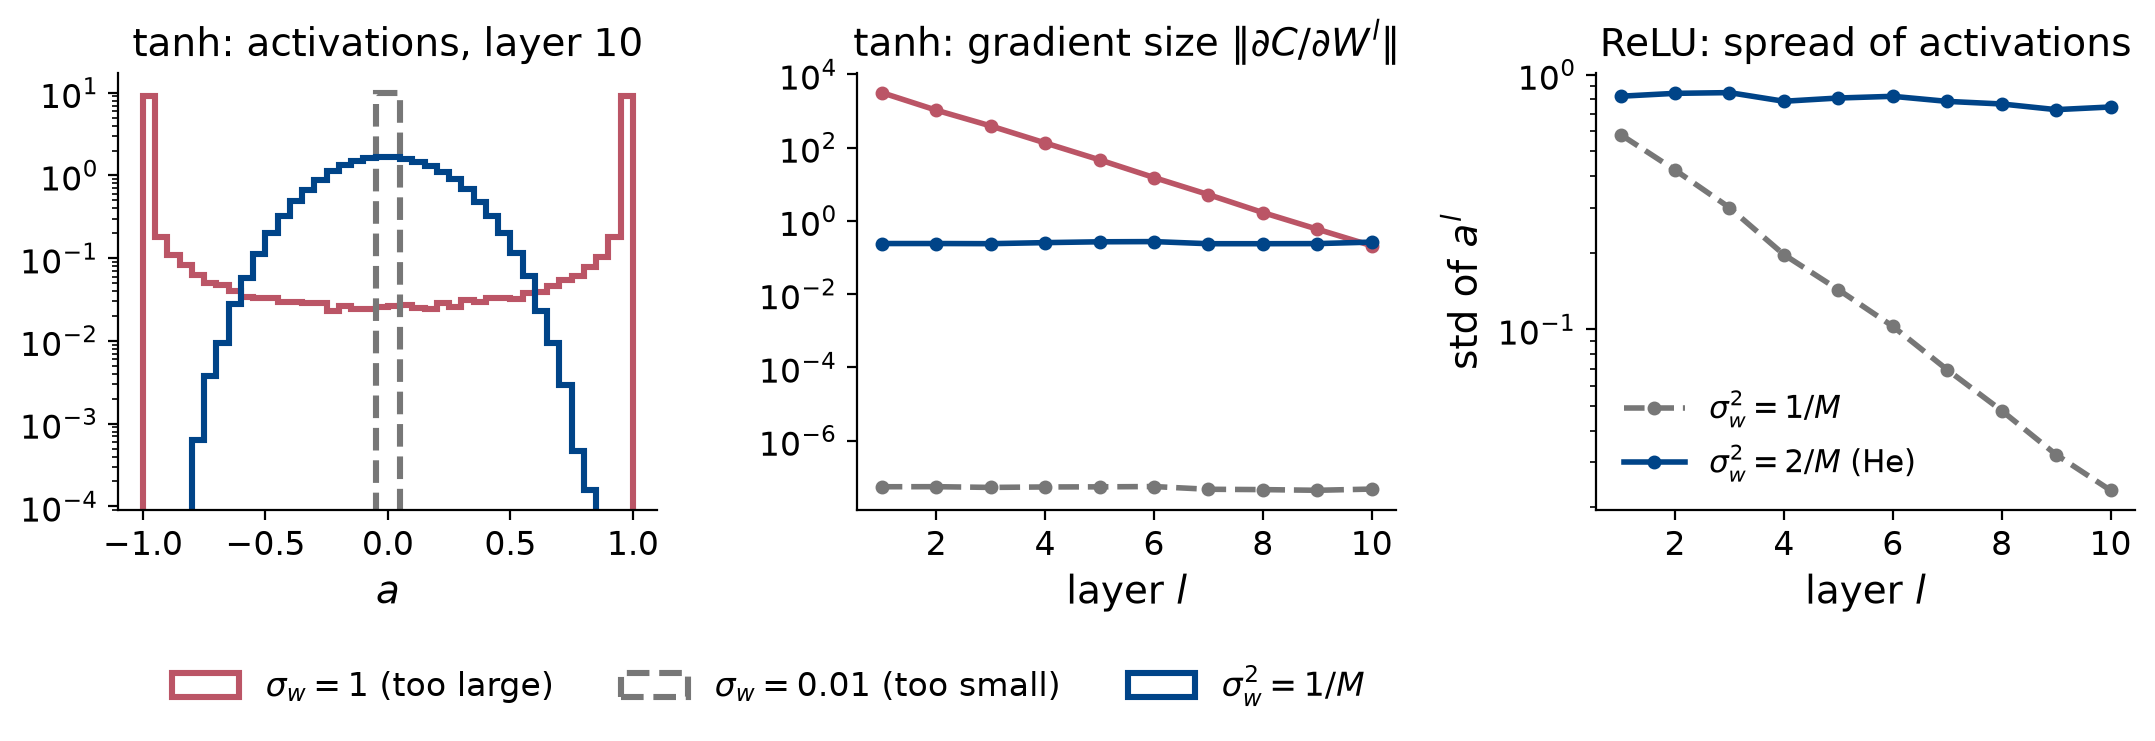
\includegraphics[width=\textwidth]{v2_init}\par
\raggedright
\small A network with 10 hidden layers of 256 units, random inputs, before
any training.
\begin{itemize}
  \item \textbf{Left:} with $\sigma_w=1$ almost all tanh units sit at
        $\pm1$ (saturated); with $\sigma_w=0.01$ everything is close to $0$.
  \item \textbf{Middle:} the gradients grow by a factor $10^{4}$ from layer
        10 to layer 1 ($\sigma_w=1$), or are tiny everywhere
        ($\sigma_w=0.01$).  With $\sigma_w^{2}=1/M$ they are the same size
        in every layer.
  \item \textbf{Right:} for ReLU, $1/M$ is not enough; $2/M$ keeps the
        signal alive.
\end{itemize}
\end{frame}

\begin{frame}{Output activation and cost function come in pairs}
\begin{center}
\setlength{\tabcolsep}{6pt}
\begin{tabular}{@{}llll@{}}
\toprule
Task & Output activation & Cost (one sample) & $\bm{\delta}^{L}$\\
\midrule
regression, $y\in\mathbb{R}$ & linear, $a=z$ & $\tfrac12(a-y)^{2}$ & \uncover<2->{$a-y$}\\[2pt]
binary, $y\in\{0,1\}$ & sigmoid, $a=\sigma(z)$ & $-y\ln a-(1-y)\ln(1-a)$ & \uncover<2->{$a-y$}\\[2pt]
$K$ classes, $\bm{y}$ one-hot & softmax, $a_k=\frac{e^{z_k}}{\sum_le^{z_l}}$ & $-\sum_ky_k\ln a_k$ & \uncover<2->{$\bm{a}-\bm{y}$}\\
\bottomrule
\end{tabular}
\end{center}
\begin{columns}[T]
\begin{column}{0.48\textwidth}
\small
\begin{itemize}
  \item The \textbf{output activation} gives the right \emph{range}: any
        real number, a probability, or $K$ probabilities that sum to one.
  \item The \textbf{cost} matches it: each is the negative log-likelihood of
        a Gaussian, Bernoulli or categorical distribution.
\end{itemize}
\end{column}
\begin{column}{0.5\textwidth}
\begin{boardbox}{W2}
Compute $\delta^{L}=f'(z)\,\dfrac{\partial C}{\partial a}$ for the sigmoid
with cross entropy.
\end{boardbox}
\pause
\begin{block}{The connection}
$f'$ \emph{cancels} against $\partial C/\partial a$:
\[
  \boxed{\;\bm{\delta}^{L}=\bm{a}^{L}-\bm{y}\;}
\]
prediction minus target, for all three pairs.
\end{block}
\end{column}
\end{columns}
\end{frame}

\begin{frame}{What goes wrong with a mismatched pair: sigmoid $+$ squared error}
\centering
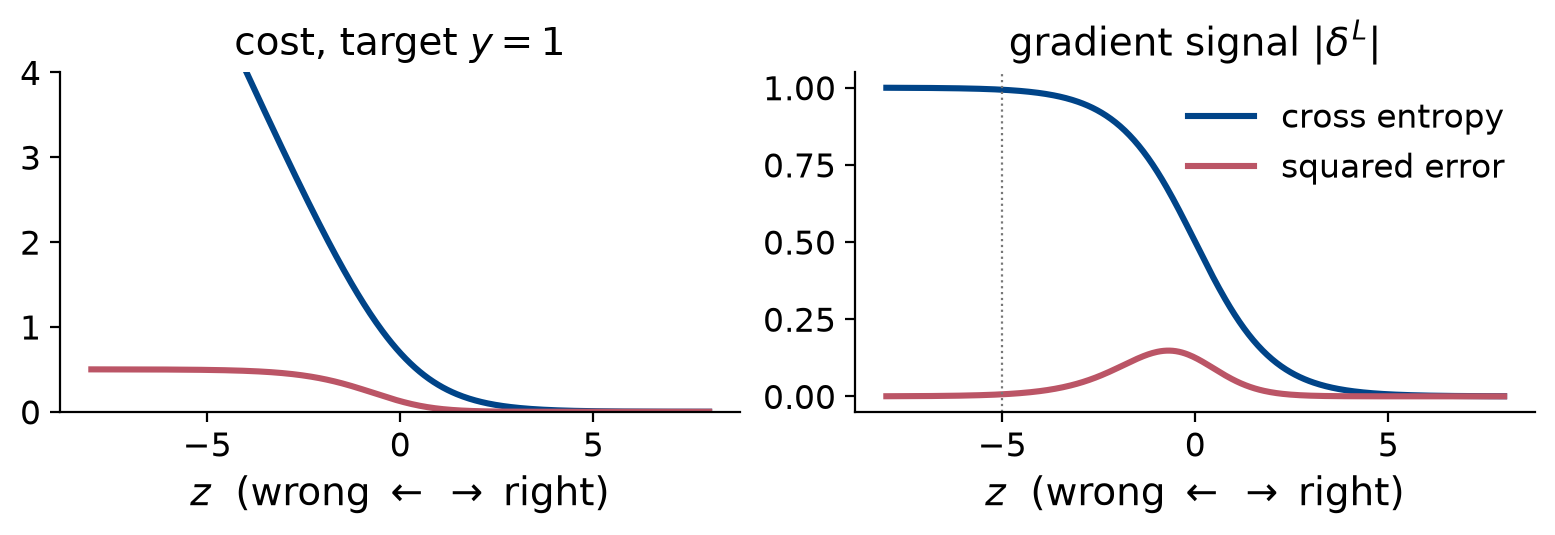
\includegraphics[width=0.78\textwidth]{v2_delta_heads}\par
\raggedright
\begin{columns}[T]
\begin{column}{0.48\textwidth}
Without the cancellation:
\[
  \delta^{L}=(a-y)\,\sigma'(z)=(a-y)\,a(1-a).
\]
\end{column}
\begin{column}{0.5\textwidth}
\small
Target $y=1$, but $z=-5$: confidently wrong, $a=0.0067$.\\[3pt]
cross entropy: $\delta=-0.993$\\
squared error: $\delta=-0.0066$, \textbf{150 times smaller}.
\end{column}
\end{columns}
\vspace{4pt}
\begin{block}{}
With the squared error, the more confidently wrong the network is, the
\emph{less} it learns.  With the cross entropy it learns the most.
\end{block}
\end{frame}

\begin{quickq}[which image trains the network?]
\begin{columns}[c]
\begin{column}{0.56\textwidth}
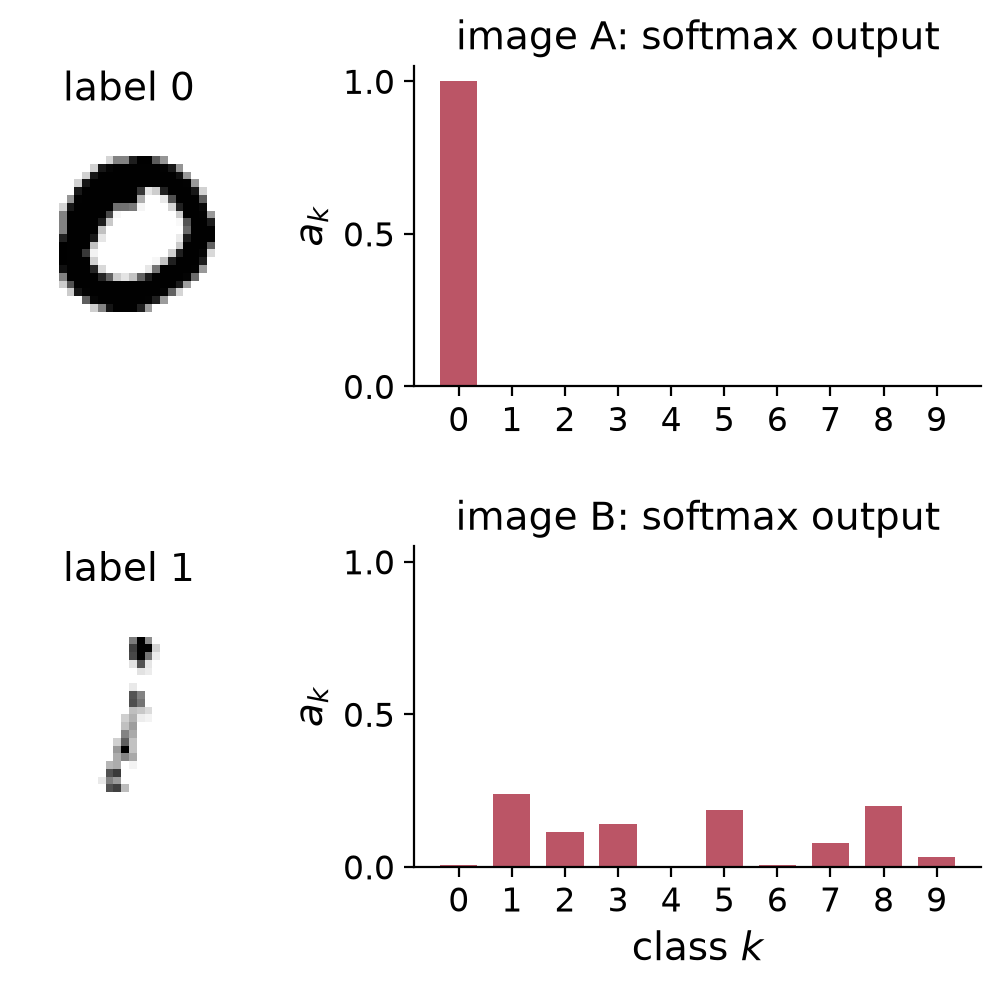
\includegraphics[width=\textwidth]{v2_mnist_question}
\end{column}
\begin{column}{0.42\textwidth}
\question{A network trained on handwritten digits (softmax $+$ cross
entropy) sees images A and B.  Using
$\bm{\delta}^{L}=\bm{a}^{L}-\bm{y}$: which image changes the weights more?}
\answer{A: $\bm{\delta}^{L}\approx\bm{0}$, nothing left to learn.\\
B: $\delta_1=0.24-1=-0.76$, and $+0.20$, $+0.19$, \dots\ for the other
classes.  Raise the score of class 1, lower the rest.\\[3pt]
The network learns from what it gets wrong or is unsure about.}
\end{column}
\end{columns}
\end{quickq}

%% ====================================================================
%% Part 3: universal approximation
%% ====================================================================

\section{Universal approximation}

\begin{frame}{The universal approximation theorem}
\begin{block}{In words}
A network with \textbf{one hidden layer} and a \textbf{non-linear}
(non-polynomial) activation can approximate \textbf{any continuous
function} on a bounded domain \textbf{as accurately as we want}, if the
hidden layer is wide enough.
\end{block}
\vspace{6pt}
\begin{columns}[T]
\begin{column}{0.46\textwidth}
\begin{block}{What it says}
\begin{itemize}
  \item A network \emph{can} represent the function we are after.
  \item The non-linearity is essential.
\end{itemize}
\end{block}
\end{column}
\begin{column}{0.5\textwidth}
\begin{block}{What it does \emph{not} say}
\begin{itemize}
  \item \emph{How many} units are needed.
  \item Whether training \emph{finds} the weights.
  \item How well it generalises to new data.
\end{itemize}
\end{block}
\end{column}
\end{columns}
\vspace{4pt}
\small Why deep networks, then?  Depth can do the same job with far fewer
units.
\end{frame}

\begin{frame}{Why it works, in one dimension: ReLU units are kinks}
\begin{columns}[T]
\begin{column}{0.5\textwidth}
\small
One ReLU unit $v\,\mathrm{ReLU}(wx+b)$ is zero, then a straight line: one
\emph{kink}, at $x=-b/w$.
\begin{boardbox}{W3}
Build a ``hat'' from three ReLU units.  Then build any curve from hats.
\end{boardbox}
\pause
\[
  \mathrm{ReLU}(x)-2\,\mathrm{ReLU}(x-1)+\mathrm{ReLU}(x-2)
\]
\centering
\begin{tikzpicture}[x=1.0cm,y=0.8cm]
  \draw[->,gray] (-0.5,0) -- (3.3,0) node[right,font=\scriptsize]{$x$};
  \foreach \t in {1,2} \draw[gray] (\t,0.05) -- (\t,-0.05) node[below,font=\scriptsize]{$\t$};
  \draw[very thick,structure.fg] (-0.5,0) -- (0,0) -- (1,0.5) -- (2,0) -- (3.2,0);
\end{tikzpicture}\par
\raggedright
Hats at $N$ points $=$ connect-the-dots.  More units, smaller error.
\end{column}
\begin{column}{0.48\textwidth}
\onslide<2->{
\centering
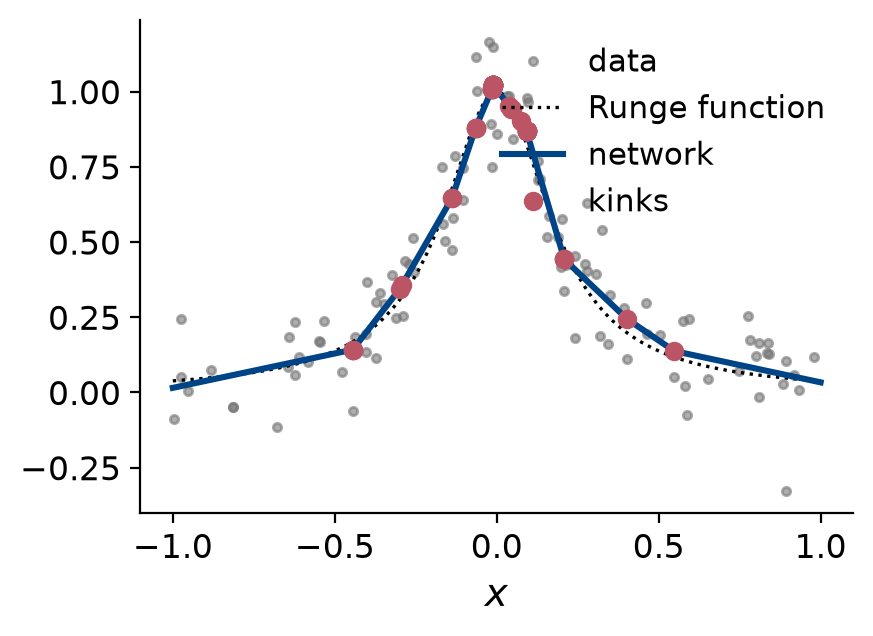
\includegraphics[width=\textwidth]{v2_runge_kinks}\par
\raggedright\small Training finds this by itself: a network with 50 ReLU
units fitted to noisy data from the Runge function.  The output is
piecewise linear, and the kinks (red) sit where the function bends.}
\end{column}
\end{columns}
\end{frame}

%% ====================================================================
%% Part 4: differential equations
%% ====================================================================

\section{Neural networks for differential equations}

\begin{frame}{Motivation: seeing the invisible}
\centering
We can film dye moving in a flow.  Can a network work out the
\emph{pressure}?\\[6pt]
%% figure from the paper; white boxes hide its panel letters B and C
\begin{tikzpicture}[
  lbl/.style={align=left,font=\small,text width=2.9cm,anchor=west},
  >={Stealth[length=5pt]}]
  \node[inner sep=0,anchor=south west] (img)
    {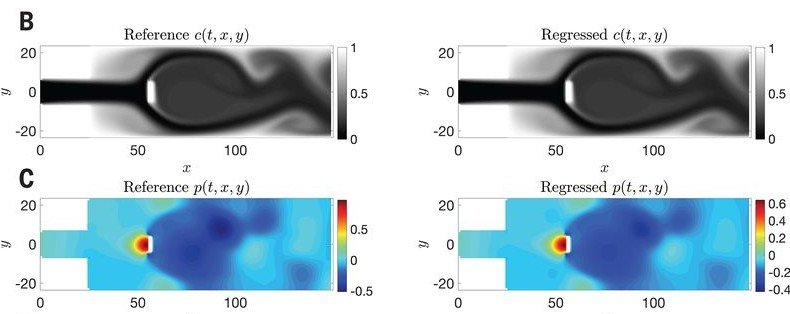
\includegraphics[width=0.72\textwidth]{hfm_cylinder}};
  \begin{scope}[x={(img.south east)},y={(img.north west)}]
    \fill[white] (0,0.89) rectangle (0.05,1);
    \fill[white] (0,0.37) rectangle (0.05,0.50);
    \node[lbl] (c) at (1.04,0.74) {\textbf{dye}\\trained on this};
    \node[lbl] (p) at (1.04,0.22) {\textbf{pressure}\\never shown,\\found by the network};
    \draw[->] (c.west)--++(-0.03,0);
    \draw[->] (p.west)--++(-0.03,0);
    \node[font=\small\bfseries] at (0.27,1.03) {simulation};
    \node[font=\small\bfseries] at (0.76,1.03) {network};
  \end{scope}
\end{tikzpicture}\\[10pt]
\raggedright
\textbf{Application:} blood flow in brain aneurysms.  Pressure and stress on
the vessel wall from a medical scan, with no probe inside the patient.\\[6pt]
\scriptsize
M.~Raissi, A.~Yazdani, G.~E.~Karniadakis, \emph{Hidden fluid mechanics},
Science \textbf{367}, 1026 (2020).
\end{frame}

\begin{frame}{A network without data: the equation is the cost}
\begin{columns}[T]
\begin{column}{0.52\textwidth}
\small
\textbf{Problem:} $g'(x)=-\kappa g(x)$, $g(0)=g_0$.  Nobody gives us data
$g(x_i)$, only the equation.\\[4pt]
\textbf{Three ingredients:}
\begin{enumerate}
  \item A \textbf{trial solution} that satisfies the conditions for
        \emph{any} network $N$:
        \[
          g_t(x)=h(x)+B(x)\,N(x),
        \]
        $h$ satisfies the conditions, $B=0$ where they are imposed.
  \item The \textbf{residual}: $r(x)=g_t'(x)+\kappa g_t(x)$, zero for the
        exact solution.
  \item The \textbf{cost}: the mean squared residual at points $x_i$ we
        choose ourselves (\emph{collocation points}),
        \[
          C=\frac1n\sum_{i=1}^{n}r(x_i)^{2}.
        \]
\end{enumerate}
\end{column}
\begin{column}{0.46\textwidth}
\begin{block}{What is new}
The residual contains $g_t'$, so we need $\partial N/\partial x$: a
derivative with respect to the \emph{input}, not the weights.  In code:
automatic differentiation (\texttt{jax.grad} with respect to $x$).
\end{block}
\begin{block}{What is not new}
Network, optimiser and backpropagation for the weights.  It is regression
with ``target'' $r=0$.
\end{block}
\end{column}
\end{columns}
\end{frame}

\begin{frame}{Example: exponential decay}
\begin{columns}[T]
\begin{column}{0.5\textwidth}
\small
$g'=-\kappa g$, $g(0)=g_0$, with $\kappa=2$, $g_0=10$.  Exact solution:
$g=g_0e^{-\kappa x}$.
\begin{boardbox}{W4}
Build $g_t$, compute $g_t'$, write the residual and the cost.
\end{boardbox}
\pause
\[
  g_t=g_0+x\,N(x),\qquad
  r=\underbrace{N+x\,N'}_{g_t'}+\kappa\,(g_0+x\,N)
\]
$g_t(0)=g_0$ whatever the network does.
\end{column}
\begin{column}{0.48\textwidth}
\onslide<2->{
\centering
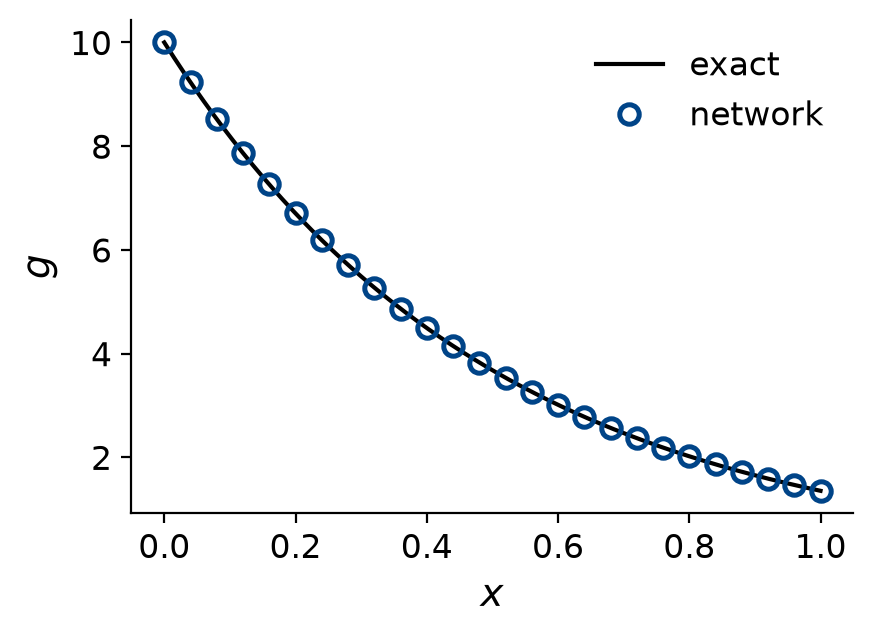
\includegraphics[width=0.9\textwidth]{v2_ode_decay}\par
\raggedright\small Two hidden layers of 40 tanh units, 50 collocation
points: max error $3\times10^{-3}$.}
\end{column}
\end{columns}
\end{frame}

\begin{frame}{The activation function matters even more now}
\begin{columns}[T]
\begin{column}{0.54\textwidth}
\small
Poisson, diffusion and wave equations contain \emph{second} derivatives,
so we need $N''(x)$.
\begin{boardbox}{W5}
Differentiate a one-hidden-layer network
$N(x)=\sum_jv_j\,f(w_jx+b_j)+c$ twice with respect to $x$.
\end{boardbox}
\pause
\[
  N''(x)=\sum_jv_j\,w_j^{2}\,f''(w_jx+b_j)
\]
\end{column}
\begin{column}{0.44\textwidth}
\onslide<2->{
\begin{block}{ReLU: $f''=0$, so $N''=0$}
A ReLU network is piecewise linear: \emph{no curvature}, for any weights.
It cannot solve $-g''=f$.
\end{block}
\small
$\max|N''|$ of a randomly initialised network:\\[3pt]
\begin{tabular}{@{}lr@{}}
\toprule
tanh & $2.9$\\
GELU & $1.2$\\
sigmoid & $0.06$\\
ReLU & $\mathbf{0}$\\
\bottomrule
\end{tabular}\\[4pt]
\textbf{We use tanh:} smooth, and $f'=1-f^{2}$, $f''=-2ff'$ are cheap.}
\end{column}
\end{columns}
\end{frame}

\begin{frame}{Boundary conditions built into the trial solution}
\begin{columns}[T]
\begin{column}{0.5\textwidth}
\small
Recipe: $g_t=h(x)+B(x)\,N(x)$, where $h$ satisfies the conditions and
$B=0$ wherever a condition is imposed.
\begin{boardbox}{W6}
Build $g_t$ for each set of conditions, and check them.
\end{boardbox}
\pause
\begin{center}
\setlength{\tabcolsep}{4pt}
\begin{tabular}{@{}ll@{}}
\toprule
Conditions & Trial solution $g_t$\\
\midrule
$g(0)=g(1)=0$ & $x(1-x)\,N$\\
$g(0)=a,\;g(1)=b$ & $a+(b-a)x+x(1-x)\,N$\\
$g(0)=g_0,\;g'(0)=v_0$ & $g_0+v_0x+x^{2}N$\\
\bottomrule
\end{tabular}
\end{center}
\end{column}
\begin{column}{0.48\textwidth}
\onslide<2->{
\begin{block}{The good}
The conditions hold \emph{exactly}, for any weights: at the start, and
after every step.  The optimiser only has to solve the equation.
\end{block}
\begin{block}{The bad}
$g_t$ must be designed by hand for every problem.  A condition on the
derivative, like $g'(1)=0$, or a curved domain: hard or impossible.
\end{block}}
\end{column}
\end{columns}
\end{frame}

\begin{frame}{Results against standard methods}
\centering
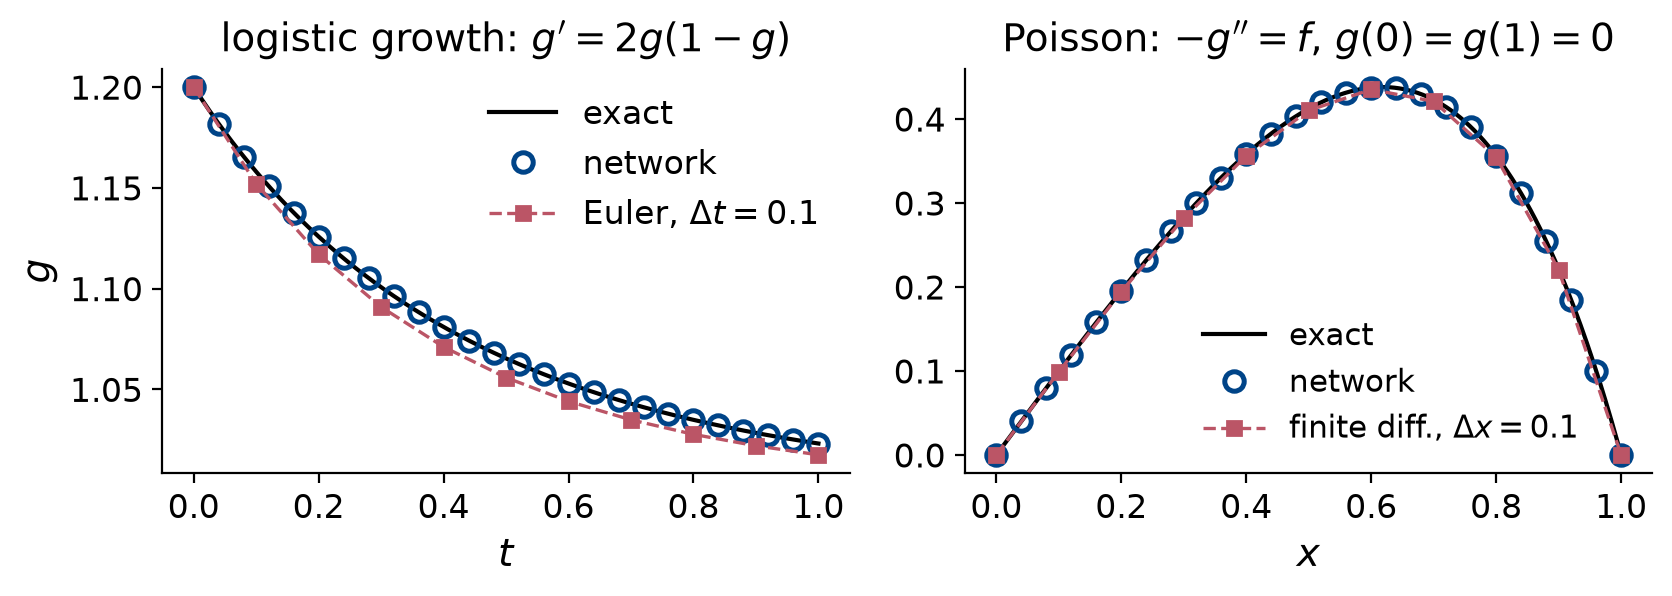
\includegraphics[width=0.8\textwidth]{v2_ode_results}\par
\raggedright
\begin{columns}[T]
\begin{column}{0.52\textwidth}
\small
Logistic growth is a \emph{non-linear} equation, but has the same trial
solution $g_0+xN$; only the residual changes.\\[4pt]
\footnotesize
\begin{tabular}{@{}lr@{\qquad}lr@{}}
\toprule
\multicolumn{2}{@{}l}{Logistic, max error} & \multicolumn{2}{l@{}}{Poisson, max error}\\
\midrule
Euler, $\Delta t=0.01$ & $9\times10^{-4}$ & FD, $\Delta x=0.01$ & $2\times10^{-5}$\\
network & $1\times10^{-4}$ & network & $1\times10^{-5}$\\
\bottomrule
\end{tabular}
\end{column}
\begin{column}{0.46\textwidth}
\begin{block}{Read it honestly}
The network is accurate.  But Euler and finite differences take
\emph{microseconds}, the network thousands of training steps.  For simple
equations like these the standard methods win.
\end{block}
\end{column}
\end{columns}
\end{frame}

\begin{frame}{A partial differential equation: diffusion}
\begin{columns}[T]
\begin{column}{0.46\textwidth}
\[
  \frac{\partial g}{\partial t}=\frac{\partial^{2}g}{\partial x^{2}},\qquad
  \begin{aligned}g(0,t)&=g(1,t)=0,\\ g(x,0)&=\sin\pi x.\end{aligned}
\]
\small The network now has \emph{two inputs}, $N(x,t)$.  Nothing else
changes.
\end{column}
\begin{column}{0.52\textwidth}
Three conditions, one trial solution:
\[
  \boxed{\;g_t=(1-t)\sin\pi x+x(1-x)\,t\,N(x,t)\;}
\]
\small Check: $t=0$ gives $\sin\pi x$; $x=0$ and $x=1$ give $0$.
\end{column}
\end{columns}
\vspace{2pt}
\centering
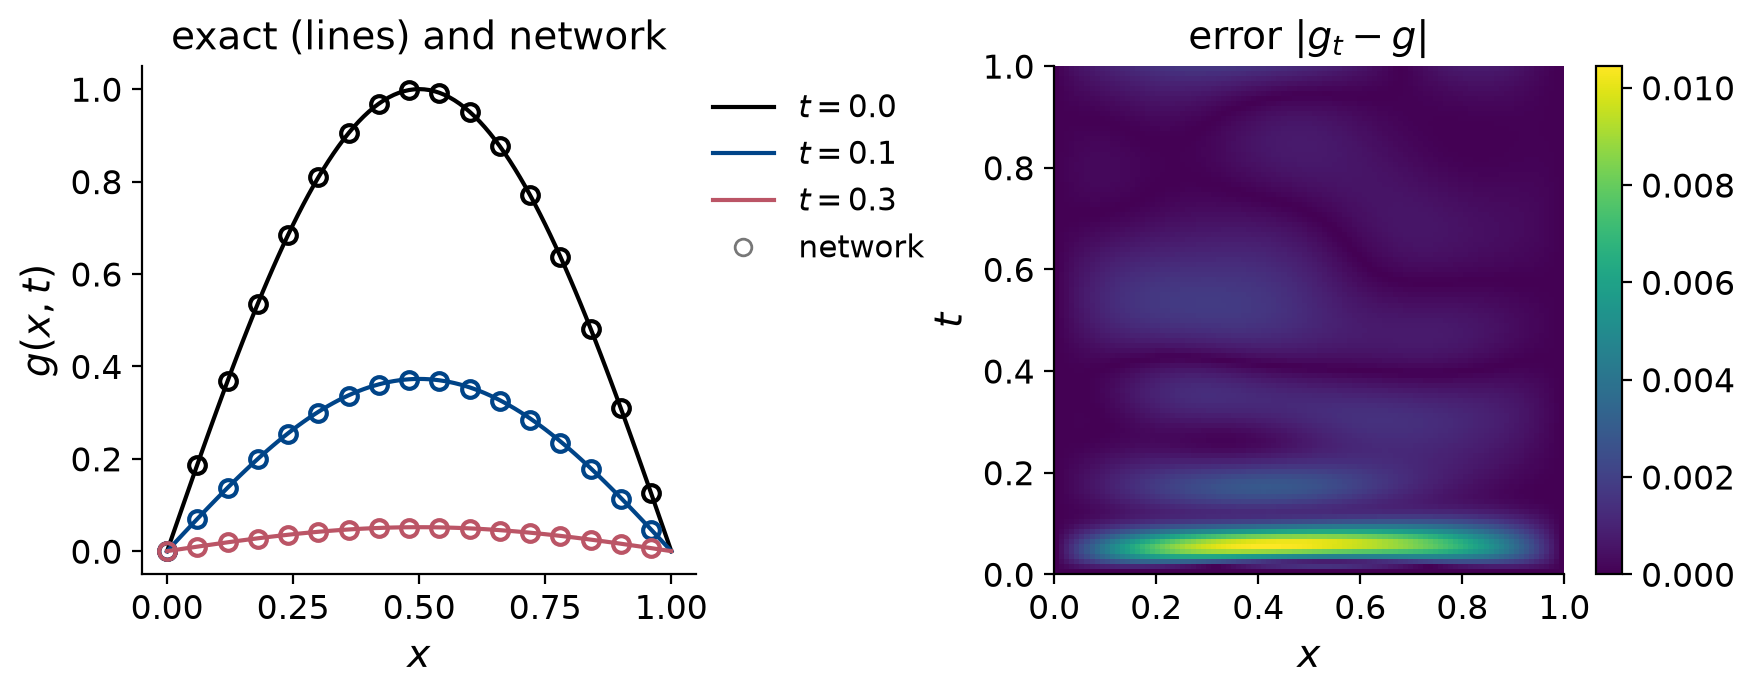
\includegraphics[width=0.74\textwidth]{v2_diffusion}\par
\raggedright\small
The error is exactly zero on the three edges (built into $g_t$), and
largest near $t=0$, where the solution changes fastest: max error
$1\times10^{-2}$.  A standard finite-difference scheme gets
$1.5\times10^{-3}$, in milliseconds.
\end{frame}

\begin{frame}{Soft constraints: physics-informed neural networks (PINNs)}
\begin{columns}[T]
\begin{column}{0.52\textwidth}
\small
Instead of building $g_t$ by hand: let the network \emph{be} the solution,
$u\approx N(x,t)$, and add the conditions to the cost as penalties:
\[
  L=L_{\mathrm{PDE}}+\lambda\,(L_{\mathrm{IC}}+L_{\mathrm{BC}})
\]
\footnotesize
\vspace{-8pt}
\begin{align*}
  L_{\mathrm{PDE}}&=\tfrac1{n}\textstyle\sum_i(\partial_tN-\partial_x^{2}N)^{2}
     &&\text{inside the domain}\\
  L_{\mathrm{IC}}&=\tfrac1{n}\textstyle\sum_i(N(x_i,0)-\sin\pi x_i)^{2}
     &&\text{at }t=0\\
  L_{\mathrm{BC}}&=\tfrac1{n}\textstyle\sum_i\bigl(N(0,t_i)^{2}+N(1,t_i)^{2}\bigr)
     &&\text{at }x=0,1
\end{align*}
\small
A new condition is just a new term.  $\lambda$ weighs the terms, like the
penalty in Ridge regression.
\end{column}
\begin{column}{0.46\textwidth}
\small
\begin{center}
\begin{tabular}{@{}lcc@{}}
\toprule
& RMSE & error at $t=0$\\
\midrule
hard ($g_t$) & $1.8\times10^{-3}$ & $0$ exactly\\
soft, $\lambda=10$ & $6.5\times10^{-3}$ & $6\times10^{-3}$\\
\bottomrule
\end{tabular}
\end{center}
\begin{block}{Hard or soft?}
\begin{itemize}
  \item If you \emph{can} build a trial solution, do: exact and more
        accurate.
  \item Soft is flexible, but the conditions hold only approximately.
  \item $\lambda$ must be tuned.  Too large, and the optimiser neglects the
        equation.
\end{itemize}
\end{block}
\end{column}
\end{columns}
\end{frame}

\begin{frame}{Why soft constraints at all?  Inverse problems}
\begin{columns}[T]
\begin{column}{0.4\textwidth}
\small
$\partial_tu=D\,\partial_x^{2}u$ with \textbf{$D$ unknown}.  No initial or
boundary conditions, only $40$ noisy measurements $y_i$.\\[4pt]
Treat $D$ as one more trainable parameter:
\begin{align*}
  L(N,D)&=\tfrac1n\textstyle\sum_j\bigl(\partial_tN-D\,\partial_x^{2}N\bigr)^{2}_j\\
  &\quad+\lambda\tfrac1{40}\textstyle\sum_i\bigl(N(x_i,t_i)-y_i\bigr)^{2}
\end{align*}
No trial solution is possible here: soft constraints are the only option.
\end{column}
\begin{column}{0.58\textwidth}
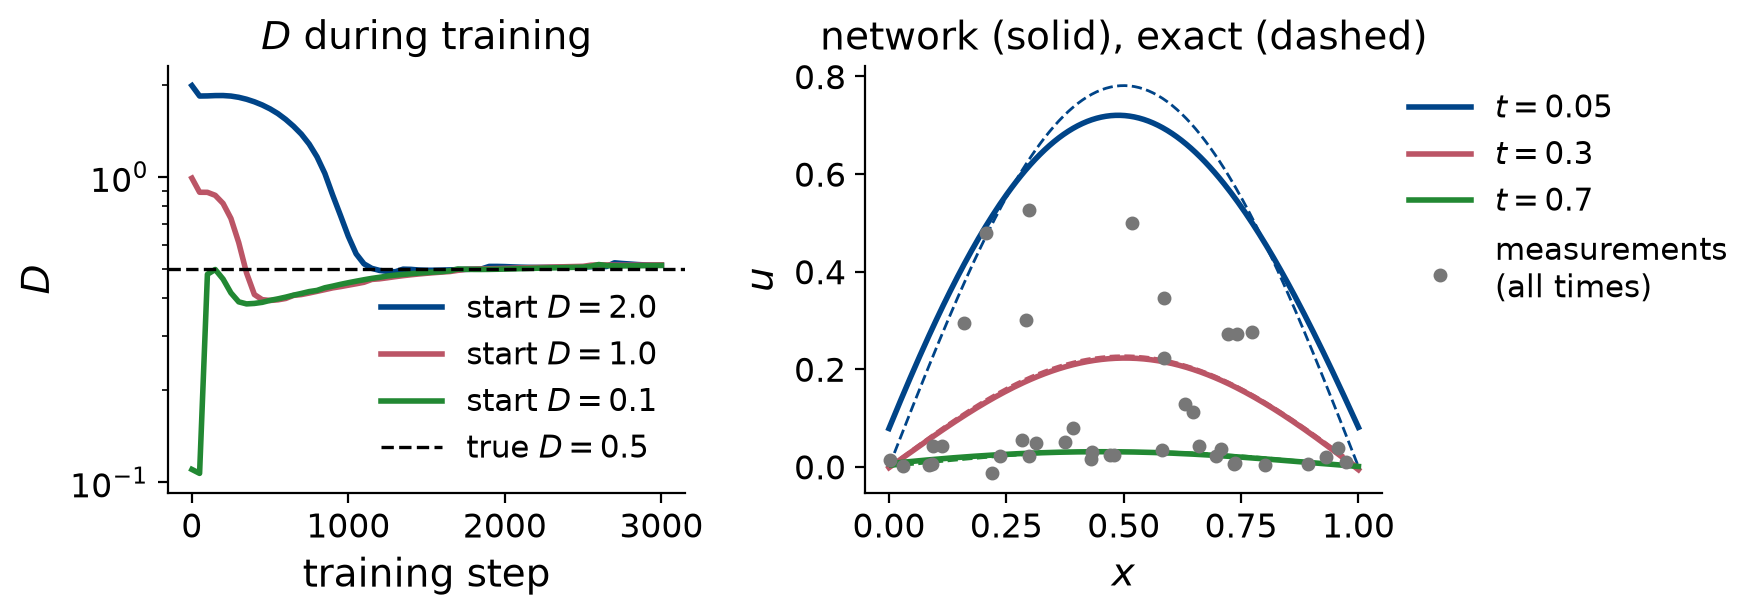
\includegraphics[width=\textwidth]{v2_pinn_inverse}\par
\small
True $D=0.5$.  Three different starting guesses all give $D\approx0.51$.
\textbf{But} with five times more noise: $D=0.69$.  A recovered parameter
needs an error bar.
\end{column}
\end{columns}
\end{frame}

\begin{frame}{Neural networks versus standard methods}
\begin{columns}[T]
\begin{column}{0.49\textwidth}
\begin{block}{Advantages}
\small
\begin{itemize}
  \item \textbf{No mesh}: complicated geometries are easy.
  \item \textbf{High dimensions}: a mesh grows exponentially with the
        dimension, random points do not.
  \item \textbf{The solution is a function}: evaluate and differentiate it
        anywhere.
  \item \textbf{Non-linear equations} need no extra work.
  \item \textbf{Data and equations together}: unknown parameters, inverse
        problems.
\end{itemize}
\end{block}
\end{column}
\begin{column}{0.49\textwidth}
\begin{block}{Disadvantages}
\small
\begin{itemize}
  \item \textbf{Slow}: thousands of training steps vs.\ microseconds.
  \item \textbf{No error guarantees} like ``error $\propto\Delta x^{2}$''.
  \item \textbf{Local minima}: can converge to a wrong answer.
  \item \textbf{Hyperparameters}: architecture, learning rate,
        $\lambda$.
  \item \textbf{Smooth activations needed}: no ReLU for second-order
        equations.
\end{itemize}
\end{block}
\end{column}
\end{columns}
\vspace{6pt}
\textbf{Bottom line:} simple problems in one or two dimensions: use
standard methods.  Networks pay off in high dimensions, complicated
geometries and inverse problems.  \textbf{Always compare with something.}
\end{frame}

\begin{frame}{Summary}
\begin{itemize}
  \item \textbf{Backpropagation} is the chain rule: compute the errors
        $\bm{\delta}^{l}$ from the output backwards; weight gradient $=$
        error $\times$ incoming signal.
  \item \textbf{Hidden activations} must be non-linear; training sees $f'$.
  \item \textbf{Output activation and cost come in pairs}, and then
        $\bm{\delta}^{L}=\bm{a}^{L}-\bm{y}$.
  \item \textbf{Universal approximation}: a wide enough network can
        represent any continuous function, but the theorem says nothing
        about size or training.
  \item \textbf{Differential equations}: the residual is the cost.
        Conditions go into the trial solution (hard) or the cost (soft).
        Use smooth activations.  Flexible, but slower than standard
        methods and without their guarantees.
\end{itemize}
\vspace{4pt}
\begin{block}{Next}
\textbf{Tuesday:} backpropagation in code.  \textbf{Exercises week 42:}
Friday October 16.  \textbf{Project 2:} November 6.
\end{block}
\end{frame}

\end{document}
